\documentclass[a4paper, 12pt, twoside]{article}
\usepackage[utf8]{inputenc}		% LaTeX, comprend les accents !
\usepackage[T1]{fontenc}		
\usepackage[francais]{babel}
\usepackage{lmodern}
\usepackage{ae,aecompl}
\usepackage[top=2.5cm, bottom=2cm, 
			left=3cm, right=2.5cm,
			headheight=15pt]{geometry}
\usepackage{graphicx}
\usepackage{eso-pic}	% Nécessaire pour mettre des images en arrière plan
\usepackage{array} 
\usepackage{hyperref}
\usepackage{subcaption}
\captionsetup[subfigure]{labelformat=empty}
\input{pagedegarde}


\title{Normalisation et nettoyage de données}
\entreprise{Le nom de votre entreprise}
\datedebut{17 octobre 2025}
\datefin{6 janvier 2026}

\membrea{Zhou Elodie 45015107}
\membreb{Hureau Massalou Georges 45007456}


\begin{document}
\pagedegarde
\section*{Remerciements}
Nous remercions Monsieur Delbot pour son encadrement, ses conseils et sa disponibilité tout au long de la réalisation de ce projet. Ses remarques nous ont permis de mieux structurer notre réflexion et d’améliorer la qualité de notre travail.

Nous remercions également l’équipe pédagogique de la formation MIAGE pour les connaissances apportées durant ce semestre.
\newpage

\tableofcontents
\newpage

\section{Introduction}
Dans un contexte où les organisations collectent des volumes croissants de données provenant de sources multiples, la qualité et la cohérence de ces données deviennent des enjeux majeurs. Les bases de données hétérogènes — issues de pays, de systèmes ou de formats différents — présentent souvent des problèmes structurels et sémantiques : incohérences de formats, valeurs manquantes, doublons, unités variables, types incorrects ou encore présence de caractères parasites.

À ces difficultés s’ajoutent les erreurs de saisie effectuées par les utilisateurs ou les clients, qui sont particulièrement fréquentes dans les systèmes d’information. Ces mauvaises saisies peuvent engendrer des conséquences importantes pour les entreprises, allant de la dégradation de la qualité des analyses jusqu’à des risques juridiques liés au non-respect de certaines obligations réglementaires. Par ailleurs, des données incorrectes ou mal normalisées peuvent provoquer des dysfonctionnements applicatifs, générer des erreurs de traitement et impacter négativement la productivité des employés, confrontés à des bugs ou à des incohérences récurrentes.

Ces irrégularités nuisent ainsi à la fiabilité des analyses, à l’intégration des systèmes d’information et à la mise en place de modèles décisionnels ou prédictifs. Dans ce contexte, la correction rapide et systématique des données apparaît comme un levier essentiel : intervenir en amont permet d’éviter l’accumulation d’anomalies au fil du temps et de prévenir une dégradation progressive de la base de données, qui deviendrait alors complexe et coûteuse à corriger a posteriori.

Le projet présenté dans ce rapport s’inscrit dans cette problématique. Il consiste à concevoir et implémenter un pipeline complet de nettoyage, correction et standardisation de bases de données internationales. L’objectif est d’être capable d’intégrer plusieurs sources de données afin d’obtenir un ensemble homogène, exploitable et conforme aux standards de qualité requis pour les traitements en aval.

Ce projet revêt également une dimension méthodologique. Au-delà de la partie technique, il vise à montrer comment des outils d’automatisation et, plus largement, l’usage de l’intelligence artificielle peuvent faciliter et améliorer les processus de préparation des données. L’IA a notamment permis de guider certaines décisions de normalisation, de détecter des irrégularités et de proposer des règles de transformation cohérentes.

Ainsi, ce travail apporte une contribution à la problématique de la data quality et de l’intégration de données hétérogènes, en mettant en œuvre des méthodes robustes et reproductibles, tout en illustrant l’intérêt d’une approche assistée par l’IA dans un contexte de nettoyage de données à grande échelle.

\newpage
\section{Environnement de travail}
Le développement du projet a été réalisé dans un environnement pour faciliter la manipulation de données, l’automatisation des tâches de nettoyage ainsi que l’export des résultats. L’ensemble du pipeline
\footnote{Un pipeline est une chaîne automatisée d’étapes successives pour déployer/traiter du code/des données.} a été implémenté en Python.

Le projet a initialement été développé et testé sur des systèmes d’exploitation Windows 11 et Linux, afin d’assurer une meilleure portabilité du code. Suite à des contraintes matérielles, l’ensemble du développement a ensuite été poursuivi exclusivement sous Windows.

L’éditeur de texte principal utilisé est Visual Studio Code, choisi pour son intégration avec GitHub et ses nombreuses extensions facilitant la rédaction de code Python et l’exécution de scripts. Le suivi de version du projet est assuré par Git, avec un dépôt GitHub collaboratif permettant de conserver l’historique et de synchroniser les modifications.

\vspace{1.5cm}
\begin{figure}[htbp]
    \centering
    \begin{subfigure}{0.22\textwidth}
        \centering
        
\includegraphics[width=\linewidth]{windows11.png}
        \caption{Windows 11}
        \label{Windows}
    \end{subfigure}
    \hspace{1 cm}
    \begin{subfigure}{0.25\textwidth}
        \centering
        
\includegraphics[width=\linewidth]{tux.png}
        \caption{Linux}
        \label{Tux}
    \end{subfigure}
    \caption{Systèmes d'exploitation utilisés}
    \label{OS}
\end{figure}
\vspace{1.5cm}
\begin{figure}[htbp]
    \centering
    \begin{subfigure}{0.25\textwidth}
        \centering
        
\includegraphics[width=\linewidth]{VSCode.png}
        \caption{VSCode}
        \label{VSCcode}
    \end{subfigure}
    \hspace{1.5 cm}
    \begin{subfigure}{0.25\textwidth}
        \centering
        
\includegraphics[width=\linewidth]{Python.png}
        \caption{Python}
        \label{Python}
    \end{subfigure}
    \hspace{1.5 cm}
    \begin{subfigure}{0.25\textwidth}
        \centering
        
\includegraphics[width=\linewidth]{github.png}
        \caption{GitHub}
        \label{Github}
    \end{subfigure}
    \caption{Outils de développement utilisés}
    \label{outils_dev}
\end{figure}

\newpage
\section{Description du projet et objectifs}
Le projet consiste à concevoir et implémenter un système complet de nettoyage, de transformation et de standardisation de données hétérogènes. En général, les données proviennent de sources multiples, sont structurées différemment et présentent des formats incompatibles. Ces variations rendent difficile l’intégration des informations dans un système unique ainsi que l’exploitation analytique ou décisionnelle.
L’objectif principal du projet est donc de mettre en place un pipeline fiable, automatisé et extensible, capable d’harmoniser plusieurs jeux de données afin de faciliter leur utilisation ultérieure.

Plus précisément, le projet vise à traiter plusieurs types d’anomalies courantes avec des données réelles :
\begin{itemize}
    \item la présence de doublons;
    \item des valeurs manquantes ou mal renseignées;
    \item des colonnes vides ou jugées inutiles pour l’analyse;
    \item des types de données incorrects (textes contenant des nombres, dates non reconnues, etc.);
    \item des incohérences textuelles telles que des espaces multiples, des caractères invisibles ou des données écrites dans des unités différentes;
    \item la coexistence de formats internationaux divergents (par exemple, virgule ou point décimal, formats de date ou d’unité variés).
\end{itemize}

L'objectif est de développer un outil générique et robuste capable d’être utilisé sur différents formats de données. Cet outil doit produire une base propre, cohérente et homogène.

\vspace{1 cm}
\begin{figure}[h]
\centering
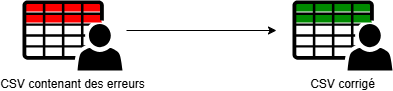
\includegraphics[scale=0.7]{Figure1.png}
\caption{Simplification visuelle}
\label{Simplif}
\end{figure}
\vspace{1 cm}

Dans le cadre de ce projet, un agent intelligent a été implémenté afin d’automatiser et d’assister le processus de nettoyage et de standardisation des données. Cet agent, implémenté dans le fichier \textit{agent\_csv}, constitue un élément central du pipeline, puisqu’il agit comme intermédiaire entre les données brutes, les règles de normalisation et l’utilisateur final.

Le rôle principal de l’agent est d’analyser un fichier CSV dès sa lecture afin d’identifier les anomalies structurelles et sémantiques présentes dans les données. Cette analyse porte sur les erreurs de données courantes présentées ci-dessus. L’agent s’appuie sur des règles prédéfinies ainsi que sur l’observation des occurrences au sein des colonnes pour détecter ces irrégularités.

Une fois les anomalies identifiées, l’agent ne procède pas directement à la modification des données. Il propose d’abord un ensemble d’opérations de correction adaptées, en s’appuyant sur le module \textit{operations}, qui regroupe l’ensemble des fonctions de nettoyage et de normalisation développées dans le cadre du projet. Ce module constitue une bibliothèque d’actions standardisées (suppression de doublons, correction des types, nettoyage des espaces, gestion des valeurs manquantes, etc.) que l’agent peut mobiliser selon les besoins détectés.

Un aspect fondamental du fonctionnement de l’agent réside dans l’intégration d’un contrôle utilisateur. Avant l’application de chaque opération de correction, l’agent sollicite explicitement la validation de l’utilisateur. Cette approche permet de conserver une supervision humaine sur les transformations appliquées aux données, réduisant ainsi les risques de pertes d’information ou de normalisations inappropriées. Elle s’inscrit dans une logique d’assistance plutôt que d’automatisation totale.

Pour s'adapter aux besoins de certains nettoyages de données, de nouvelles règles peuvent être implémentées dans \textit{operations}, permettant à l'agent de les apprendre rapidement et automatiquement. La séparation claire entre l’analyse effectuée par \textit{agent\_csv} et les règles définies dans \textit{operations} permettent d’enrichir progressivement le système.

Ainsi, l’agent intelligent joue un rôle clé dans la structuration du pipeline de nettoyage, en combinant automatisation, modularité et validation humaine, tout en illustrant l’apport potentiel de l’IA dans les processus de préparation et de qualité des données.

\section{Bibliothèques, Outils et technologies}
Dans le cadre de ce projet, différents outils et technologies ont été mobilisés afin
de faciliter le développement et la standardisation des bases de données. Plusieurs bibliothèques Python sont utilisées pour les traitements :
\begin{itemize}
    \item \textbf{pandas} pour la manipulation, la structuration et l’analyse des tables de données ;
    \item \textbf{datetime} pour la gestion des dates lors de l’export des fichiers ;
    \item \textbf{os} pour la gestion des dossiers et fichiers.
    \item \textbf{sys} : pour interagir avec l’environnement d’exécution, notamment pour la gestion des arguments, des chemins et du comportement du programme.
    \item \textbf{requests} : permet d’effectuer des requêtes HTTP de manière simple et efficace, utilisée pour communiquer avec des services externes ou des API, notamment dans le cadre de l’agent intelligent.
    \item \textbf{json} : pour la lecture, l’écriture et la manipulation de données au format JSON, facilitant l’échange d’informations structurées entre les différents modules du projet.
    \item \textbf{numpy} : pour le calcul numérique, utilisée pour la manipulation efficace de tableaux de données et le traitement de valeurs numériques au sein des opérations de nettoyage et d’analyse.
\end{itemize}
Les données manipulées sont principalement stockées au format CSV, choisi pour sa simplicité, sa lisibilité et sa compatibilité avec de nombreux outils d’analyse. Le format JSON est également utilisé pour structurer certaines informations intermédiaires et faciliter les échanges entre les différents modules.

L’ensemble de ces bibliothèques et technologies permet de construire un système modulaire et adapté au traitement de données hétérogènes.

\newpage
\section{Travail réalisé}

\subsection*{Fonctionnalités réalisées}

Les fonctionnalités suivantes ont été implémentées et sont opérationnelles dans la version finale du projet :
\begin{itemize}
    \item Connexion à un agent d’intelligence artificielle (Mistral IA).
    \item Analyse automatique des fichiers CSV par l’agent IA afin de détecter les anomalies.
    \item Application d’opérations de nettoyage et de normalisation des données.
    \item Confirmation des opérations de nettoyage avant leur application.
    \item Génération d’un fichier CSV nettoyé, distinct du fichier original.
    \item Statistiques en fin de traitement afin de synthétiser les opérations effectuées.
\end{itemize}

\subsection*{Fonctionnalités non réalisées}

La reprise automatique des valeurs \textit{``n/a''} à l’aide d’un système de comparaison au sein d’une même colonne n’a pas été implémentée. Le principe envisagé consistait à détecter une valeur manquante sur une ligne donnée, puis à proposer plusieurs valeurs possibles issues des autres lignes de la colonne, tout en laissant la possibilité à l’utilisateur de saisir une valeur personnalisée ou de conserver \textit{``n/a''}.

La détection d’incohérences inter-colonnes, par exemple une valeur \textit{Pays = France} associée à une \textit{Devise = USD}, n’a également pas été implémentée. L’identification exhaustive de ce type d’incohérences et la définition des opérations de correction adaptées se sont révélées complexes et particulièrement chronophages. Nous n’avons pas trouvé de solution générique et efficace permettant de traiter l’ensemble de ces cas de manière fiable.

Enfin, l’ajout dans le rapport d’un indicateur chiffré de qualité des données, exprimé en pourcentage avant et après traitement, n’a pas pu être implémenté. Les valeurs de fiabilité proposées par l’intelligence artificielle n’étaient pas cohérentes avec les données analysées ni avec les résultats obtenus après nettoyage. En l’absence d’un indicateur fiable et objectif, il a été décidé de ne pas intégrer cette fonctionnalité afin d’éviter toute interprétation erronée.

\subsection*{Répartition du travail}

Le travail a été réalisé de manière coopérative tout au long du projet. Les séances de développement se sont déroulées soit à la bibliothèque universitaire, soit à distance via Discord, afin de faciliter les phases de réflexion. Le code a été réalisé en peer programming sur le poste de Georges afin de favoriser une recherche conjointe des erreurs rencontrées.

Concernant la rédaction du rapport, les différentes parties ont été réparties entre les membres du groupe et rédigées sur un document partagé via Google Drive. Une fois l’ensemble des sections finalisées, le contenu a été regroupé et harmonisé sur Overleaf.

\newpage
\section{Apport de l’intelligence artificielle dans le projet}

L’intelligence artificielle a joué un rôle central tout au long de la réalisation de ce projet, aussi bien sur le plan conceptuel que technique. Le domaine du nettoyage et de la standardisation des bases de données étant relativement nouveau pour les membres du groupe, ce projet constituait une première expérience de travail approfondi avec des données structurées.

Dans un premier temps, l’IA a été mobilisée pour aider à la réflexion et à la conception du projet. Elle a permis de clarifier les objectifs, d’identifier les différentes étapes du pipeline de nettoyage.

Sur le plan du développement, une grande partie du code a été générée avec l’aide de l’intelligence artificielle. Ces générations ont servi de base de travail, puis ont été analysées, adaptées et corrigées afin de répondre précisément aux besoins du projet.

L’IA a également été sollicitée pour l’aide à la résolution d’erreurs, l’explication du fonctionnement de certaines bibliothèques Python et l’amélioration de la lisibilité du code. Enfin, elle a contribué à la rédaction du rapport, notamment pour la reformulation de passages et la clarification de certaines explications.

Dans l'ensemble, l'IA a beaucoup été utilisé pour nous permettre d'avancer dans le projet et de ne pas rester bloquer par manque de connaissance dans le domaine et dans la programmation. Toutefois, les réponses fournies par l'IA ont été analysées afin de les aligner avec les objectifs fixés et la vision globale du projet.

\newpage
\section{Fonctionnement de l’agent d’intelligence artificielle et intégration des réponses dans le code}

L’agent d’intelligence artificielle intégré au projet repose sur l’utilisation de l’API Mistral AI. Il a été conçu comme un agent d’analyse et de décision, chargé d’identifier les anomalies présentes dans un fichier CSV et de proposer des opérations de nettoyage adaptées, sans modifier directement les données de manière autonome.

\subsection{Lecture et préparation des données}

Le fonctionnement de l’agent débute par la lecture du fichier CSV fourni par l’utilisateur. Cette étape est réalisée à l’aide de la bibliothèque \textit{pandas}, qui permet de charger les données sous forme de \texttt{DataFrame}. Une attention particulière est portée à la gestion des types de données dès la lecture, notamment pour certaines colonnes sensibles telles que les codes postaux, les numéros de téléphone, les identifiants ou les numéros administratifs. Ces colonnes sont explicitement forcées en type texte afin d’éviter des problèmes courants tels que la notation scientifique ou la suppression de zéros en début de valeur.

L’agent prend également en compte les différents encodages possibles des fichiers CSV (UTF-8, Latin-1, CP1252), afin d’assurer une lecture des données, même en présence de fichiers provenant de sources hétérogènes. Les chaînes vides sont ensuite remplacées par des valeurs manquantes afin de normaliser la représentation des données absentes.

\subsection{Création d’un résumé destiné à l’IA}

Une fois les données chargées, l’agent génère un résumé détaillé du fichier CSV. Ce résumé contient notamment :
\begin{itemize}
    \item le nombre de lignes et de colonnes,
    \item la liste des colonnes,
    \item les types de données détectés,
    \item le nombre de valeurs manquantes par colonne,
    \item le nombre de doublons,
    \item un échantillon des premières lignes,
    \item des statistiques descriptives globales.
\end{itemize}

Ces informations constituent une synthèse structurée du contenu du fichier et servent de base à l’analyse réalisée par l’intelligence artificielle. L’objectif est de fournir à l’agent IA une vision globale du jeu de données sans lui transmettre l’intégralité du fichier, ce qui permet de limiter le volume d’informations échangées avec l’API.

\newpage
\subsection{Résumé du prompt utilisé par l’agent \textit{agent\_csv}}

Le prompt transmis à l’API Mistral constitue un élément central du fonctionnement de l’agent intelligent. Il a été conçu afin de cadrer strictement le rôle de l’IA et de limiter les réponses incohérentes ou non exploitables par le programme.

Dans ce prompt, l’IA est explicitement définie comme un agent spécialisé dans l’analyse et le nettoyage de données tabulaires au format CSV. Elle reçoit un résumé structuré du fichier à analyser, incluant les informations générales sur le jeu de données, la liste des colonnes, les types de données détectés, le nombre de valeurs manquantes, la présence éventuelle de doublons ainsi qu’un échantillon des premières lignes.

Le prompt précise également les types d’anomalies que l’IA doit rechercher en priorité, tels que :
\begin{itemize}
    \item la présence de doublons,
    \item les valeurs manquantes ou incohérentes,
    \item les problèmes de format ou de type de données,
    \item les erreurs liées aux chaînes de caractères (espaces, caractères invisibles).
\end{itemize}

Afin de garantir l’exploitabilité des réponses, le prompt impose un format de sortie strict en JSON. Chaque anomalie détectée doit être décrite à l’aide d’attributs précis, notamment le type de problème identifié, la ou les colonnes concernées, l’opération de nettoyage recommandée ainsi que les paramètres nécessaires à son exécution.

Enfin, le prompt restreint volontairement les actions possibles de l’IA en l’obligeant à s’appuyer exclusivement sur les opérations définies dans le module \textit{operations}. L’IA ne peut donc ni inventer de nouvelles règles de nettoyage, ni appliquer directement des modifications aux données. Ce choix permet de mieux contrôler le comportement de l’agent et d’assurer la cohérence entre l’analyse réalisée par l’IA et les traitements effectivement implémentés dans le projet.


\subsection{Analyse des anomalies et interprétation de la réponse}

En réponse au prompt, l’agent IA retourne une liste structurée d’anomalies détectées. Chaque anomalie est décrite à l’aide de plusieurs attributs, tels que son type, sa gravité, les colonnes concernées, l’opération de nettoyage recommandée et les paramètres associés.

Cette étape constitue le cœur du rôle de l’IA dans le projet : l’agent ne se contente pas d’identifier des erreurs, mais propose également des actions concrètes, directement exploitables par le module \textit{operations}. L’IA agit donc comme un moteur de décision, tandis que l’exécution des corrections est entièrement déléguée au code du projet.

\subsection{Validation utilisateur et exécution contrôlée}

Avant toute modification effective des données, l’agent affiche chaque anomalie détectée dans la console et demande à l’utilisateur de valider ou non l’application de la correction proposée. Cette interaction permet de conserver un contrôle humain sur le processus de nettoyage et d’éviter toute transformation non souhaitée des données.

Lorsque l’utilisateur valide une correction, l’agent appelle dynamiquement la fonction correspondante du module \textit{operations}, en lui transmettant les paramètres fournis par l’IA. Les opérations sont ainsi appliquées de manière séquentielle et contrôlée sur une copie du jeu de données.

\newpage
\section{Difficultés rencontrées}
    \subsection{Conception différente du projet}
Comme dit précédemment, nous avions des visions différentes du projet, malgré une idée commune : normaliser des bases de données.  
D’un côté, l’idée était de définir les opérations de nettoyage dans un fichier dédié, puis de faire appel à l’intelligence artificielle pour les utiliser avec les bons paramètres d’entrée.  
De l’autre côté, l’idée était de faire appel à l’IA pour détecter et corriger elle-même les anomalies présentes dans les données.

Après une phase de réflexion et de discussion, nous en avons conclu, avec la validation de Monsieur Delbot, que l’IA pouvait avoir une place importante dans le projet, notamment en analysant les données et en guidant l’utilisateur étape par étape. Afin d’éviter des variations dans les fichiers nettoyés par l’IA, nous avons mis en place un module \textit{operations} sur lequel l’agent IA s’appuie pour réaliser les corrections de manière cohérente.

    \subsection{Contraintes matérielles}
Suite à une défaillance matérielle survenue la veille d’un rendez-vous de travail, une perte partielle du travail réalisé a été constatée, entraînant l’annulation de la séance prévue. Un nouvel ordinateur a toutefois pu être utilisé dès le lendemain, ce qui a permis de reprendre rapidement le développement du projet à distance, à l’aide d’outils de communication en ligne tels que Discord. Cette adaptation a permis de maintenir une collaboration efficace malgré l’impossibilité de travailler physiquement au même endroit pendant cette période.

    \subsection{Gestion de la clé API Gemini}
Lorsque nous avons implémenté la clé API Gemini, nous avons rencontré un problème de version de la clé. Toutes nos fonctions faisant appel à l’IA produisaient une erreur. Pour résoudre ce problème, nous avons suivi les étapes indiquées par ChatGPT, mais nous n’avons pas réussi à mettre à jour la version après une heure d’essais.

C’est pourquoi nous avons choisi de passer à une clé API Mistral afin de pouvoir continuer le projet. Par la suite, nous n’avons plus rencontré de problème avec celle-ci.

    \subsection{Variabilité des réponses de l'IA}
Une fois la clé API mise en place, nous lui avons fourni un fichier CSV contenant des erreurs de doublons, des valeurs improbables et des adresses e-mail invalides afin qu’elle les corrige. Nous avons ensuite lancé plusieurs fois le programme avec le même fichier pour vérifier si l’IA nous fournissait le même fichier CSV corrigé en sortie, et ce n’était pas toujours le cas.

Cela a mis en évidence la possibilité d’obtenir des réponses différentes de l’IA. Pour corriger les données, les fonctions de standardisation ont été codées localement et l’IA se charge d’analyser le fichier CSV, de lister les anomalies et d’appliquer nos fonctions.

    \subsection{Incohérence entre l’analyse de l’agent et les résultats produits}
L’agent est capable d’identifier correctement les problèmes présents dans les données et de proposer des solutions pertinentes sous forme textuelle dans la console. Toutefois, lors de la génération du fichier CSV nettoyé, certaines modifications annoncées ne sont pas réellement prises en compte.

Ce comportement met en évidence un écart entre l’analyse réalisée par l’agent, qui est globalement correcte, et l’application concrète des opérations de nettoyage sur les données. Ainsi, bien que les recommandations formulées soient cohérentes et pertinentes, leur implémentation automatique ne reflète pas toujours fidèlement les corrections décrites. Cette difficulté a nécessité une vérification manuelle des fichiers générés et souligne les limites actuelles de l’automatisation complète du processus de nettoyage.

\newpage
\section{Bilan}
	\subsection{Conclusion}
Ce projet avait pour objectif de concevoir un outil de nettoyage et de standardisation de bases de données hétérogènes, en s’appuyant sur le langage Python et sur l’utilisation d’un agent d’intelligence artificielle. À travers ce travail, nous avons mis en place un pipeline permettant de lire des fichiers CSV, de détecter différentes anomalies et d’appliquer des opérations de correction et de normalisation de manière structurée.

Le projet nous a permis de mieux comprendre les problématiques liées à la qualité des données, notamment la gestion des doublons, des valeurs manquantes, des incohérences de formats et des erreurs de saisie. Il a également mis en évidence les limites actuelles de l’automatisation par l’intelligence artificielle, en particulier le décalage possible entre l’analyse des données et l’application effective des corrections.

Malgré certaines difficultés techniques et organisationnelles, le projet a abouti à une solution fonctionnelle, modulaire et évolutive. L’approche retenue, séparant clairement le rôle de l’agent intelligent et celui des opérations de nettoyage, constitue une base solide pour de futures améliorations et extensions.

	\subsection{Perspectives}
Plusieurs axes d’amélioration et d’évolution peuvent être envisagés pour prolonger ce projet.

Tout d’abord, l’intégration d’un mécanisme de traduction permettrait de traiter des bases de données multilingues, ce qui renforcerait l’objectif de standardisation entre des sources provenant de différents pays.

Ensuite, le projet pourrait être étendu à la gestion de bases de données relationnelles, en complément des fichiers CSV actuellement supportés. Une connexion directe à une base de données permettrait de traiter des volumes plus importants et de s’intégrer plus facilement dans des systèmes d’information existants.

Une autre perspective concerne le rôle de l’intelligence artificielle dans le processus de nettoyage. Il serait pertinent de limiter certaines opérations automatiques, telles que la suppression des doublons ou le choix de l’encodage, afin de laisser davantage de contrôle à l’utilisateur selon ses besoins et ses préférences.

L’amélioration des performances constitue également un axe important, notamment pour anticiper le traitement de jeux de données de grande volumétrie. Des optimisations techniques seraient nécessaires afin d’augmenter l’efficacité et la rapidité du pipeline.

Par ailleurs, le développement d’une interface graphique pourrait remplacer l’exécution via la console. Une telle interface améliorerait l’expérience utilisateur et rendrait l’outil plus accessible à des profils non techniques.

Enfin, à plus long terme, il serait envisageable de concevoir un agent d’intelligence artificielle dédié, capable d’apprendre progressivement à partir des corrections effectuées et des données traitées. Cette perspective reste toutefois un objectif de recherche à long terme, difficilement réalisable dans le cadre de ce projet.

\newpage
\section{Webographie}
\begin{thebibliography}{2}
    \bibitem [ChatGPT]{chatgpt} OpenAI – ChatGPT : \url{https://openai.com}
    \bibitem [Gemini]{gemini} Google – Gemini : \url{https://ai.google.dev}
    \bibitem [Mistral]{mistral} Mistral AI : \url{https://mistral.ai}
    \bibitem [Claude]{claude} Anthropic – Claude : \url{https://www.anthropic.com}
    \bibitem[Kaggle]{kaggle} Kaggle :\url{https://www.kaggle.com/datasets}
    \bibitem [Python]{docpython} Documentation Python : \url{https://docs.python.org}
    \bibitem [Pandas]{pandas} Documentation pandas : \url{https://pandas.pydata.org/docs}
    \bibitem [NumPy]{numpy} Documentation NumPy : \url{https://numpy.org/doc}
\end{thebibliography}

\newpage
\section{Annexes}
\appendix
\makeatletter
\def\@seccntformat#1{Annexe~\csname the#1\endcsname:\quad}
\makeatother
	\section{Cahier des charges}
\subsection*{Contexte}
Le projet s’inscrit dans le cadre de la formation MIAGE et vise à concevoir un outil de nettoyage et de standardisation de données hétérogènes à l’aide de Python et de l'intelligence artificielle.

\subsection*{Objectifs}
\begin{itemize}
    \item Analyser des fichiers CSV contenant des données hétérogènes.
    \item Détecter les anomalies présentes dans les données (doublons, valeurs manquantes, incohérences de format).
    \item Proposer et appliquer des opérations de nettoyage et de normalisation.
    \item Assister l’utilisateur à l’aide d’un agent intelligent.
    \item Exporter les données nettoyées dans des fichiers distincts.
\end{itemize}

\subsection*{Fonctionnalités attendues}
\begin{itemize}
    \item Lecture de fichiers CSV.
    \item Détection des doublons.
    \item Gestion des valeurs manquantes.
    \item Nettoyage des chaînes de caractères (espaces, caractères invisibles).
    \item Correction des types de données.
    \item Standardisation des formats (dates, unités).
    \item Export automatique des fichiers nettoyés avec date et heure.
\end{itemize}

\subsection*{Contraintes}
\begin{itemize}
    \item Fonctionner avec n'importe quel jeux de données.
    \item Compatibilité avec plusieurs système d'exploitation.
    \item Validation des modifications par l'utilisateur.
\end{itemize}

\subsection*{Livrables}
\begin{itemize}
    \item Code source du projet.
    \item Rapport de projet.
    \item Jeux de données de test.
\end{itemize}

\newpage
	\section{Manuel utilisateur : exemple d'exécution}
\subsection*{Présentation de l’outil}
L’outil développé dans ce projet permet de nettoyer et de standardiser des fichiers de données au format CSV. Il est conçu pour détecter automatiquement certaines anomalies (doublons, valeurs manquantes, incohérences de format) et produire un fichier nettoyé, prêt à être exploité.

\subsection*{Prérequis}
Pour utiliser l’outil, l’utilisateur doit disposer d’un environnement Python fonctionnel ainsi que d’un fichier CSV à analyser. Une connaissance de l'utilisation d'une console est nécessaire.
\begin{figure}[htbp]
    \centering
    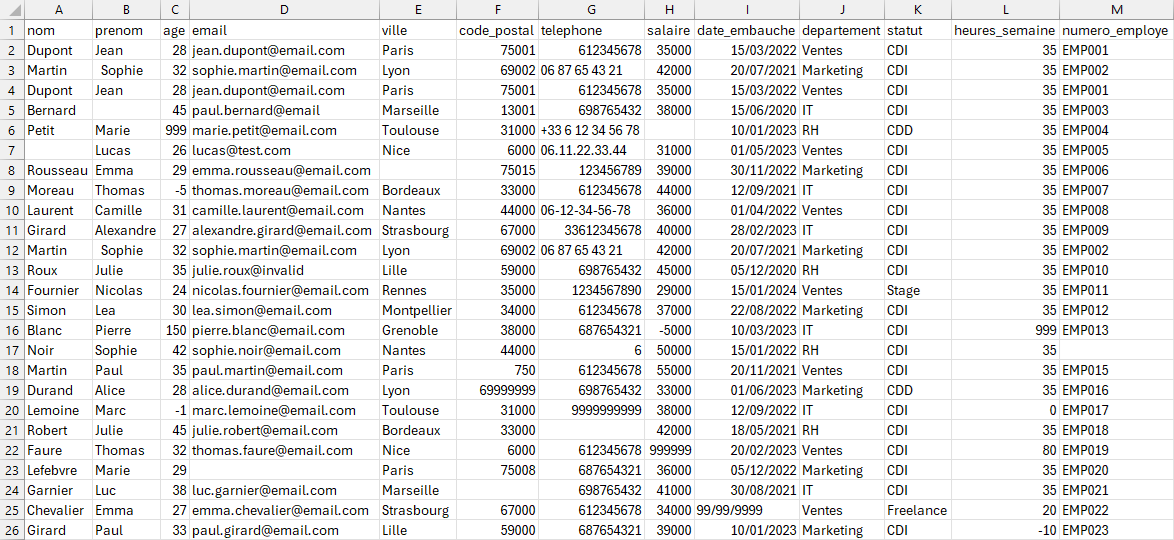
\includegraphics[width=0.8\textwidth]{capture_avant.png}
    \caption{Fichier CSV en entrée}
    \label{csv_entree}
\end{figure}

\subsection*{Utilisation}
L’utilisateur doit placer le fichier CSV à nettoyer dans le dossier \textit{Raw}. Une fois le programme lancé, l’agent analyse automatiquement le contenu du fichier et applique les opérations de nettoyage définies.
\begin{figure}[htbp]
    \centering
    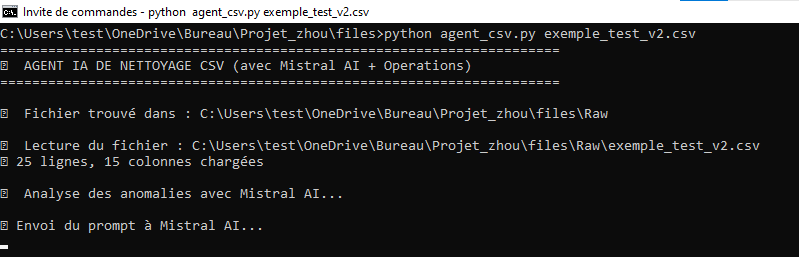
\includegraphics[width=0.8\textwidth]{capture_demarrage.png}
    \caption{Console au démarrage}
    \label{demarrage}
\end{figure}

\newpage
Durant l’exécution, des informations sont affichées dans la console afin d’indiquer les différentes étapes du traitement. À chaque étape \textit{``Appliquer cette correction ?''}, la console attend la réponse de l'utilisateur.
\begin{figure}[htbp]
    \centering
    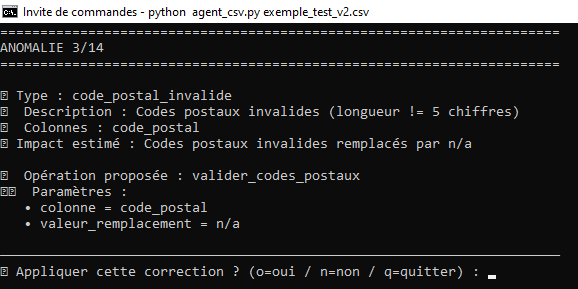
\includegraphics[width=0.6\textwidth]{capture_entree.png}
    \caption{En attente d'une réponse de l'utilisateur}
    \label{entree}
\end{figure}

\begin{figure}[htbp]
    \centering
    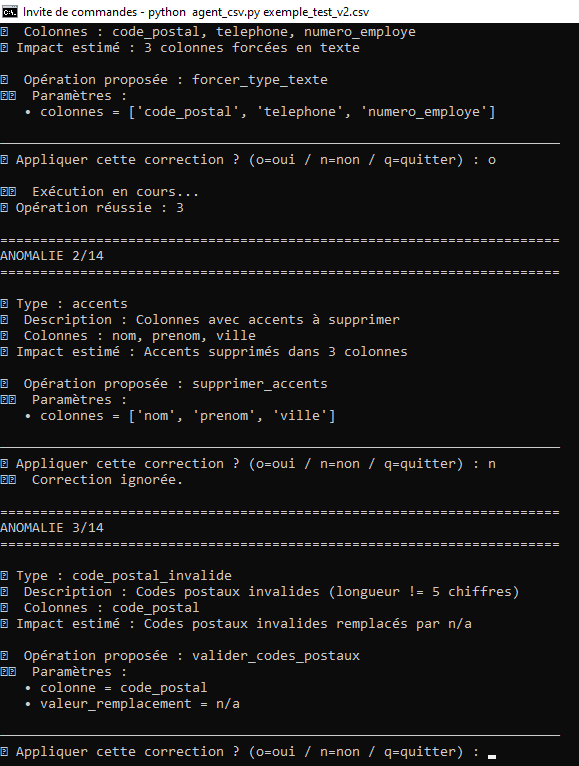
\includegraphics[width=0.6\textwidth]{capture_etapes.png}
    \caption{Etapes du nettoyage}
    \label{etapes}
\end{figure}

\newpage
L'utilisateur peut également décider de quitter le programme en cours.
\begin{figure}[htbp]
    \centering
    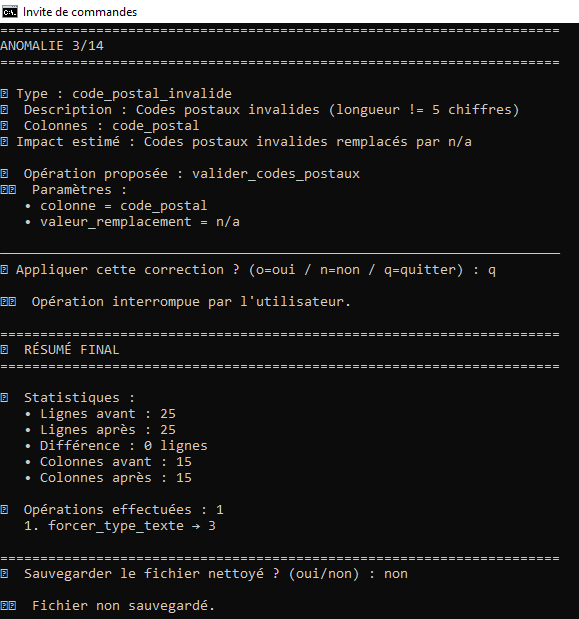
\includegraphics[width=0.8\textwidth]{capture_quitter.png}
    \caption{L'utilisateur quitte le programme}
    \label{quitter}
\end{figure}

\newpage
Une fois les étapes finalisées, le programme fourni un compte rendu d'exécution dans la console et propose de sauvegarder le fichier nettoyé.
\begin{figure}[htbp]
    \centering
    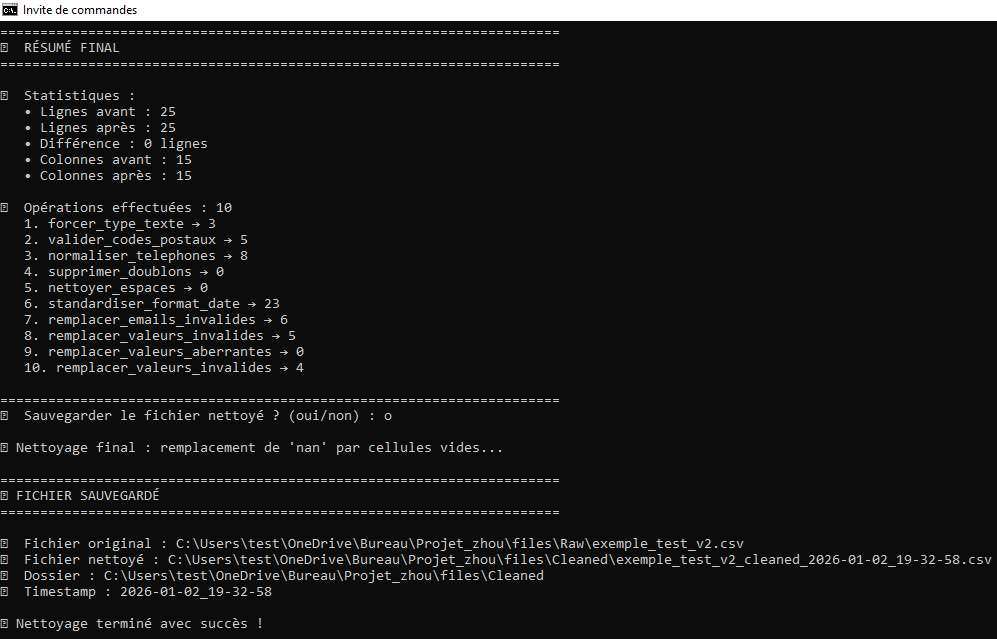
\includegraphics[width=0.8\textwidth]{capture_final.png}
    \caption{Compte rendu et demande de sauvegarde du fichier nettoyé}
    \label{final}
\end{figure}

\subsection*{Résultats}
À l’issue de l’exécution, un nouveau fichier CSV est généré. Ce fichier contient les données nettoyées et standardisées. Il est automatiquement enregistré dans un dossier dédié nommé \textit{Cleaned}. Le nom du fichier inclut la date et l’heure de génération afin d’éviter l’écrasement des résultats précédents.
\begin{figure}[htbp]
    \centering
    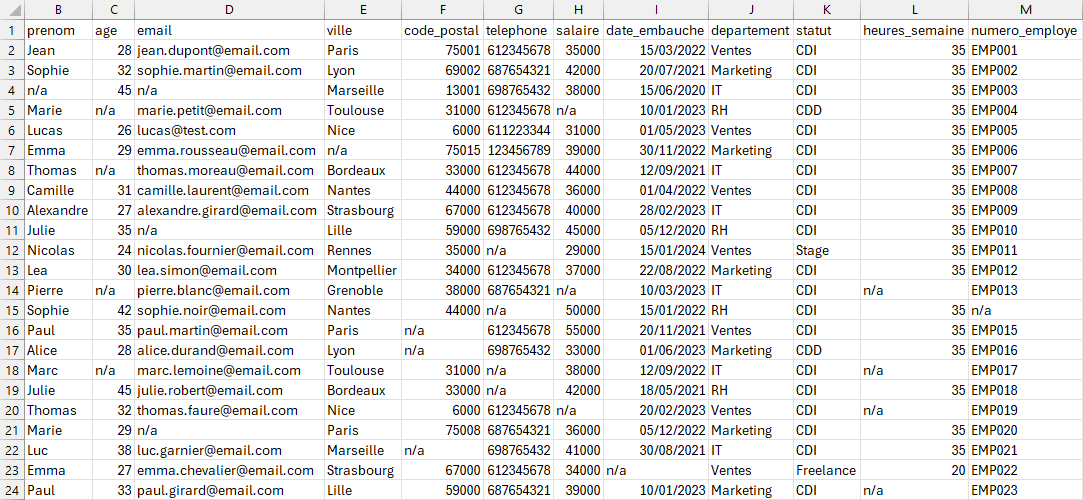
\includegraphics[width=0.8\textwidth]{capture_apres.png}
    \caption{Fichier CSV en sortie}
    \label{csv_sortie}
\end{figure}

\subsection*{Remarque}
L’outil ne modifie jamais le fichier original. L'objectif est de proposer un fichier nettoyé sans perdre les informations des données initiales.

\end{document}